


\section{Two-Element Array}
\subsection{要求}
\noindent 根据方向图乘积定理,画出不同组态的电偶极子元天线二元阵的方向图
\begin{align*}
&d=\lambda/4, \beta=0\\
&d=\lambda/4, \beta=\pi/2\\
&d=\lambda/2, \beta=0\\
&d=\lambda/2, \beta=\pi\\
&d=\lambda/2, \beta=\pi/2\\
\end{align*}	

\subsection{原理及推导}
根据电偶极子的远场特性,将其z向排阵
\begin{equation}
EF=E_\theta=j\eta\dfrac{kI_0le^{-jkr}}{4\pi r}\cos\theta
\end{equation}
\begin{equation}
(AF)_n=\cos\left[\dfrac{1}{2}(kd\cos\theta+\beta)\right]
\end{equation}
\begin{equation*}
TF=EF\times AF
\end{equation*}
归一化之后常数项没有任何影响,所以
\begin{equation}
E_{total}\simeq \cos\theta\cos\left[\dfrac{1}{2}(kd\cos\theta+\beta)\right]
\end{equation}
\subsection{结果与分析}
如图\ref{fig:2element}所示, 与教材上的结果相符合. 
\begin{figure}[!ht]
	\centering
	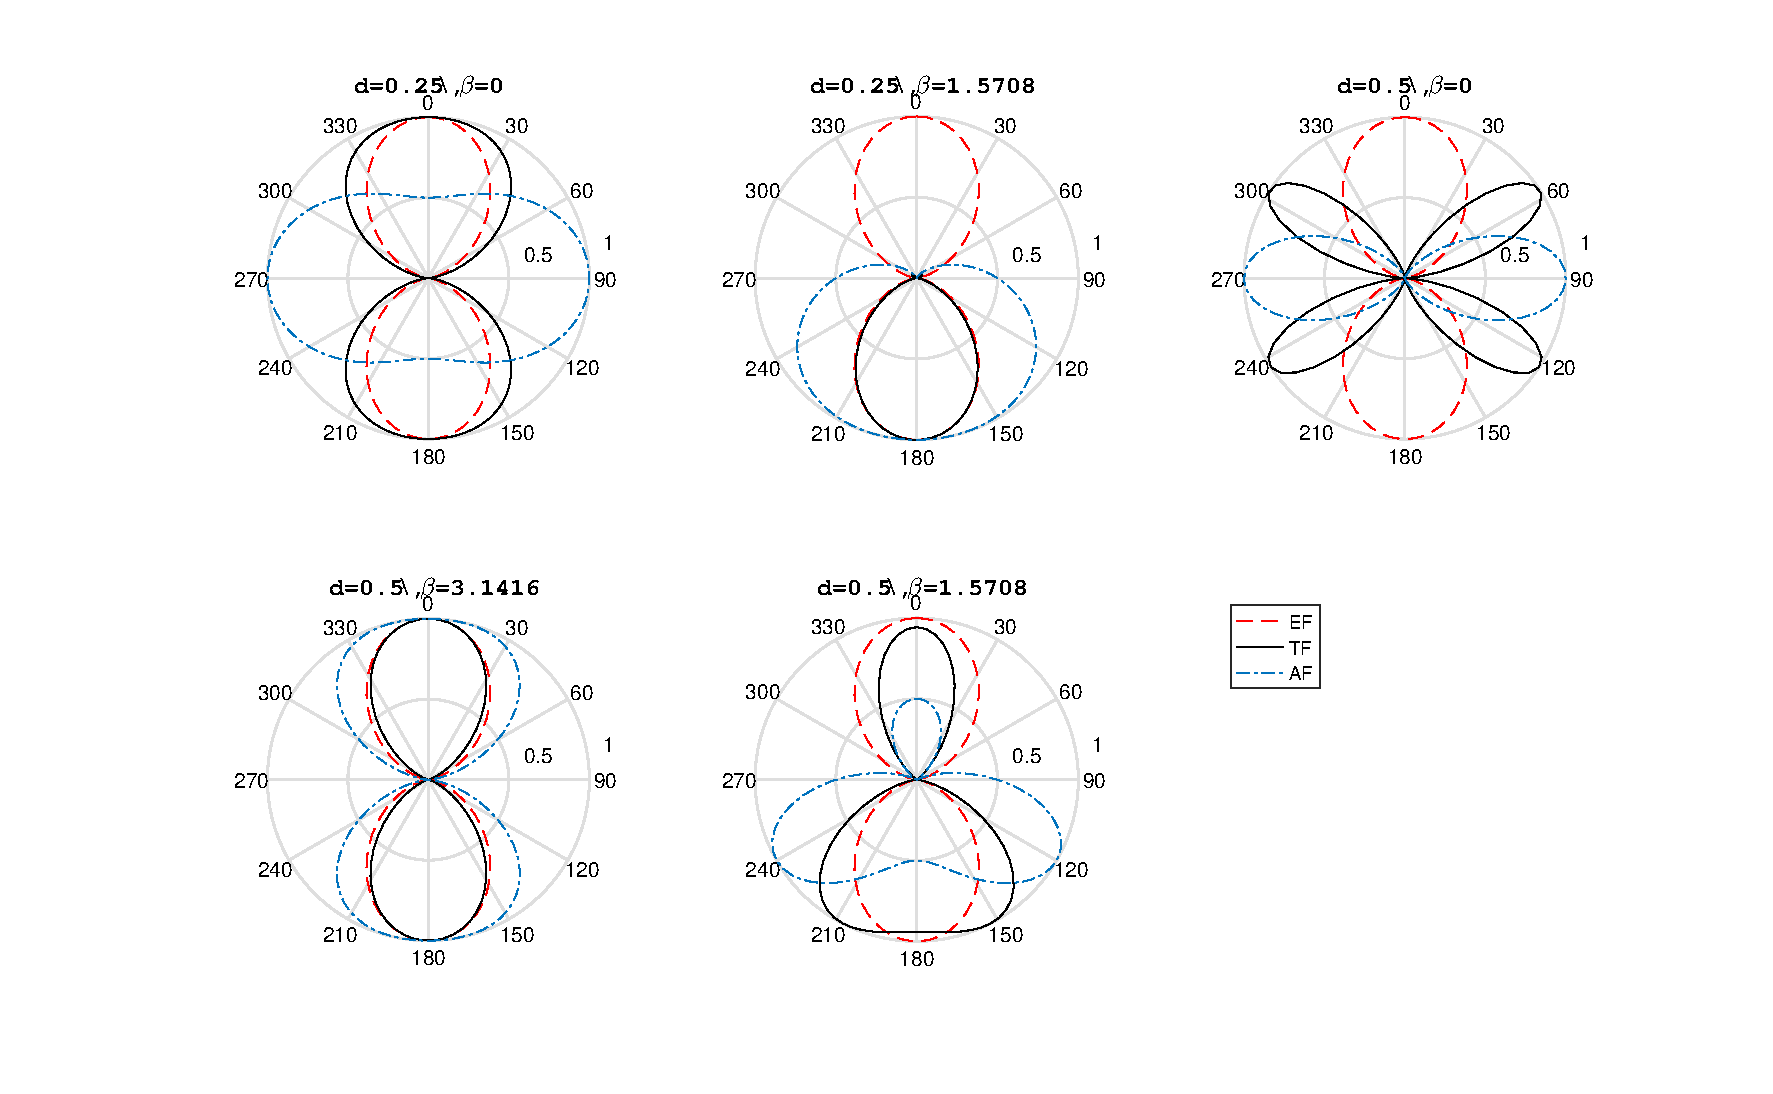
\includegraphics[width=\textwidth]{array2element.eps}
	\caption{$TF=EF\times AF$} \label{fig:2element}
\end{figure}
\newpage
\subsection{程序}
\noindent \textbf{主程序}
\begin{lstlisting}[language={matlab},keywordstyle=\color{blue!70},commentstyle=\color{red!50!green!50!blue!50},frame=shadowbox, rulesepcolor=\color{red!20!green!20!blue!20}] 
clear
close all
d=[0.25 0.25 0.5 0.5 0.5];
beta=[ 0 0.5*pi 0 pi 0.5*pi];
for i=1:5
subplot(2,3,i)
Fun_2array(d(i),beta(i))
end
subplot(2,3,6)
plot(0,0,'r--');hold on
plot(0,0,'k');hold on
plot(0,0,'-.);
axis off
legend('EF','TF','AF','Location','northwest')
\end{lstlisting}
\noindent \textbf{子函数}
\begin{lstlisting}[language={matlab},keywordstyle=\color{blue!70},commentstyle=\color{red!50!green!50!blue!50},frame=shadowbox, rulesepcolor=\color{red!20!green!20!blue!20}] 
function Fun_2array(d,beta)
%d lamda
%beta rad
%phi=kdcos(theta)+beta ??
%?????????????????????????????
theta=linspace(0,2*pi,100);
phi=2*pi*d*cos(theta)+beta;
% EF=abs(cos(theta));         %only E
% AF=abs(cos(0.5*phi));       %only E
EF=cos(theta).^2;         %power
AF=cos(0.5*phi).^2;       %power
TF=AF.*EF;
TF=TF/max(TF);
polar (theta,EF,'r--');hold on
polar(theta,TF,'k');hold on
polar(theta,AF,'-.');
view(90,-90)
% legend('EF','TF','AF','Location','northeastoutside')
titlename=strcat('d=',num2str(d),'\lambda',',', '\beta
=',num2str(beta));
title(titlename,'Fontname','TimeNewsRoman','Fontsize',
12)
end
\end{lstlisting}